\documentclass[pdf]{beamer}

\usetheme[progressbar=frametitle]{metropolis}

\usepackage[spanish]{babel}
\usepackage[utf8]{inputenc}

%\usepackage{kpfonts}
%\usepackage{inconsolata}

\usepackage[scale=2]{ccicons}

\usepackage{newunicodechar}
\newunicodechar{λ}{\lambda}
\newunicodechar{Λ}{\Lambda}
\newunicodechar{α}{\alpha}
\newunicodechar{β}{\beta}
\newunicodechar{δ}{\delta}
\newunicodechar{Δ}{\Delta}
\newunicodechar{Γ}{\Gamma}
\newunicodechar{ω}{\omega}
\newunicodechar{Ω}{\Omega}
\newunicodechar{ρ}{\rho}
\newunicodechar{σ}{\sigma}
\newunicodechar{Σ}{\Sigma}
\newunicodechar{τ}{\tau}
\newunicodechar{ν}{\nu}
\newunicodechar{μ}{\mu}
\newunicodechar{ξ}{\xi}
\newunicodechar{Ξ}{\Xi}
\newunicodechar{ζ}{\zeta}
\newunicodechar{η}{\eta}
\newunicodechar{φ}{\phi}
\newunicodechar{Φ}{\Phi}
\newunicodechar{π}{\pi}
\newunicodechar{Π}{\Pi}
\newunicodechar{θ}{\theta}
\newunicodechar{Θ}{\Theta}

\newcommand{\bs}{\boldsymbol}

\title{El cálculo \texorpdfstring{\( \bs{λ} \)}{lambda}}
\subtitle{Y los fundamentos de la computación}
\author{Eduardo Acuña Yeomans}
\institute{Universidad de Sonora}
\date{\today}
\titlegraphic{\hfill
\includegraphics[height=2cm]{escudo-unison}}

\begin{document}

\maketitle

\begin{frame}{Contenido}
  \setbeamertemplate{section in toc}[sections numbered]
  \tableofcontents%[hideallsubsections]
\end{frame}

\section{Introducción}

\begin{frame}
  \frametitle{¿Qué es el cálculo \texorpdfstring{\( \bs{λ} \)}{lambda}?}
  
  \begin{figure}
    \centering
    
\includegraphics[scale=.25]{pimg/pensando.png}
  \end{figure}
  \pause
  
  \begin{itemize}
  \item<2-> \alert<2>{Un lenguaje para expresar cómputo}
    \[ λf.(λx.f\, (x\, x))\, (λx.f\, (x\, x)) \]
  \item<3-> \alert<3>{Teoría matemática}
    \[ \bs{λKβ}, Γ \vdash M = N \]
  \item<4-> \alert<4>{Sistema para estudiar matemáticas y computación}
    \begin{figure}[!tbp]
      \centering
      \begin{minipage}[b]{0.15\textwidth}
        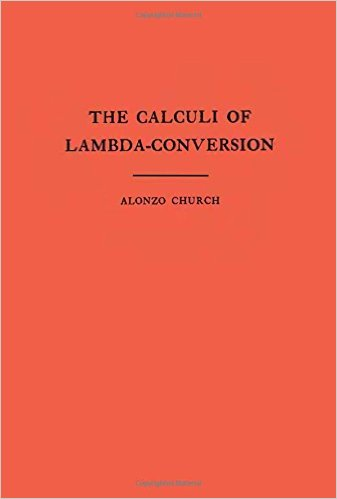
\includegraphics[width=\textwidth]{libro-church.jpg}
      \end{minipage}
      \hfill
      \begin{minipage}[b]{0.15\textwidth}
        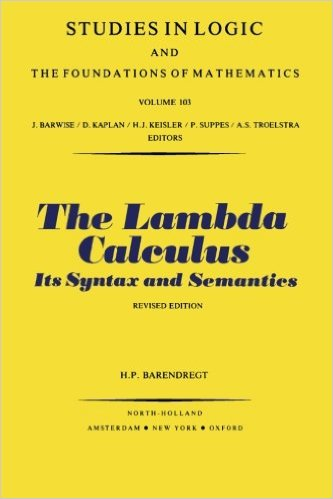
\includegraphics[width=\textwidth]{libro-barendregt.jpg}
      \end{minipage}
      \hfill
      \begin{minipage}[b]{0.15\textwidth}
        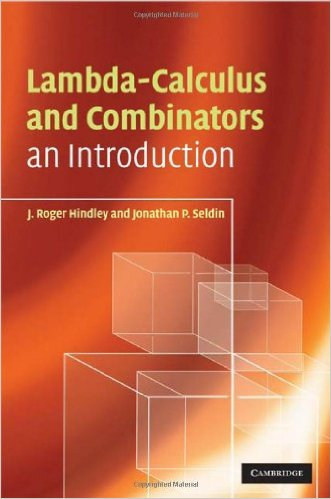
\includegraphics[width=\textwidth]{libro-hindley.jpg}
      \end{minipage}
      \hfill
      \begin{minipage}[b]{0.15\textwidth}
        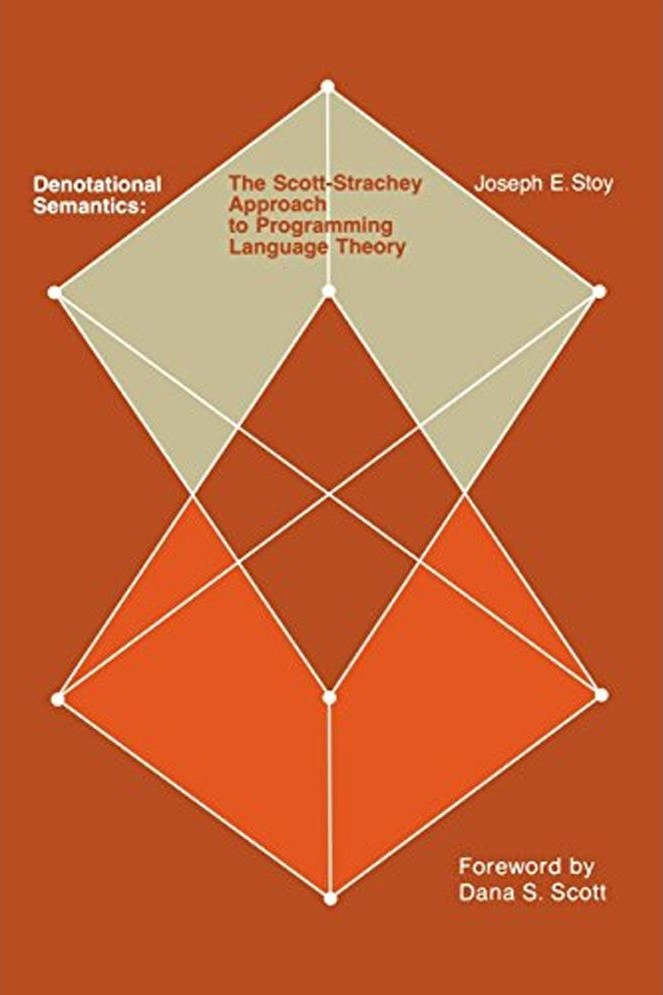
\includegraphics[width=\textwidth]{libro-stoy.jpg}
      \end{minipage}
    \end{figure}
  \end{itemize}
\end{frame}

\begin{frame}
  \frametitle{Orígen}
  \begin{minipage}[c]{.3\textwidth}
    \begin{figure}
      \centering
      \only<1>{Alonzo Church}
      
      \includegraphics<1>[scale=.2]{pimg/church.jpg}

      \only<2>{Barkley Rosser}
      
      \includegraphics<2>[scale=.2]{pimg/rosser.PNG}

      \only<2>{Stephen Kleene}
        
      \includegraphics<2>[scale=.1]{pimg/kleene.jpg}

      \only<3>{Alonzo Church}
      
      \includegraphics<3>[scale=.2]{pimg/church.jpg}
    \end{figure}
  \end{minipage}%
  \begin{minipage}[c]{.7\linewidth}
    \begin{description}[<+- | alert@+>]
    \item[1932] Un conjunto de postulados para la fundamentación de la lógica
    \item[1935] La insconsistencia de ciertas lógicas formales
    \item[1936] Un problema sin solución de la teoría de números elemental
    \end{description}
    
  \end{minipage}
  
\end{frame}

\begin{frame}
  \frametitle{Concepto de función}
  \onslide<1->{
    \[ f : A \to B \]
    \[ f(x) = E \]
    \[ f(a) = b \]
  }%
  \onslide<3->{
    \[ \{ (a,b) \mid a\in A,\ b\in B \} \]
  }%
  \onslide<2->{
    \[ \downarrow \]
    \[ f = (λx.E) \]
    \[ (f\, a) = b \]
  }%
  \onslide<3->{
    \[ (\quad λ\quad x\quad .\quad E\quad ) \]
  }
\end{frame}

\section{Conceptos básicos}

\begin{frame}
  \frametitle{Términos \texorpdfstring{\( \bs{λ} \)}{lambda}}
  
  \begin{center}
    \only<3>{\( M\in \)} \only<4>{\( M,\ N\in \)} \( Λ \)
  \end{center}
  
  \begin{itemize}
  \item \alert<2>{Variables} \hfill \onslide<2->{\( w \), \( x \), \( y \), \( z \), etc.}
  \item \alert<3>{Abstracciones} \hfill \onslide<3->{\( (λx.M) \)}
  \item \alert<4>{Aplicaciones} \hfill \onslide<4->{\( (M\, N) \)}
  \end{itemize}

  \onslide<5>{
    \begin{center}
      El alfabeto tiene como elementos los símbolos:
      
      \( (\qquad )\qquad λ\qquad . \)
    
      y a todas las variables
    \end{center}
  }
\end{frame}

\begin{frame}
  \frametitle{Términos \texorpdfstring{\( \bs{λ} \)}{lambda}}
  
  \begin{center}
    \only<1>{
      Identificando la estructura de un término \( λ \)
      \[ \textcolor{black}{(}\textcolor{black}{(}\textcolor{black}{λ}\textcolor{black}{y}\textcolor{black}{.}\textcolor{black}{(}\textcolor{black}{y}\textcolor{black}{\,}\textcolor{black}{z}\textcolor{black}{)}\textcolor{black}{)}\textcolor{black}{\,}\textcolor{black}{y}\textcolor{black}{)} \]
    }
    \end{center}
    
    \only<2>{
      Las aplicaciones tienen la forma \( (M\, N) \)
      \[ \textcolor{black}{(}\textcolor{gray}{(}\textcolor{gray}{λ}\textcolor{gray}{y}\textcolor{gray}{.}\textcolor{gray}{(}\textcolor{gray}{y}\textcolor{gray}{\,}\textcolor{gray}{z}\textcolor{gray}{)}\textcolor{gray}{)}\textcolor{gray}{\,}\textcolor{gray}{y}\textcolor{black}{)} \]
    }%
    \only<2>{
      Las abstracciones tienen la forma \( (λx.M) \)
      \[ \textcolor{gray}{(}\textcolor{black}{(}\textcolor{black}{λ}\textcolor{gray}{y}\textcolor{black}{.}\textcolor{gray}{(}\textcolor{gray}{y}\textcolor{black}{\,}\textcolor{gray}{z}\textcolor{gray}{)}\textcolor{black}{)}\textcolor{black}{\,}\textcolor{gray}{y}\textcolor{gray}{)} \]
    }%
    \only<2>{
      Las variables se clasifican por su posición en la expresión
      \[ \textcolor{gray}{(}\textcolor{gray}{(}\textcolor{gray}{λ}\textcolor{black}{y}\textcolor{gray}{.}\textcolor{gray}{(}\textcolor{black}{y}\textcolor{gray}{\,}\textcolor{black}{z}\textcolor{gray}{)}\textcolor{gray}{)}\textcolor{gray}{\,}\textcolor{black}{y}\textcolor{gray}{)} \]
      \begin{itemize}
      \item Variables vinculadas
      \item Variables ligadas
      \item Variables libres
      \end{itemize}
    }
\end{frame}

\begin{frame}
  \frametitle{Operaciones}

  Un término \( λ \) puede ser transformado a otros términos \( λ \) utilizando el concepto de \alert{sustitución}.

  \vfill
  
  \onslide<2>{
    Sustituír una variable \( x \) por un término \( N \) en un término \( M \) se denota

    \[ M[x:=N] \]
  }
  
\end{frame}

\begin{frame}
  \frametitle{Operaciones}

  Ejemplos de sustituciones

  \begin{align*}
    x[x:=(λy.y)] &\rightarrow (λy.y) \\
    x[z:=(λy.y)] &\rightarrow x \\
    (x\, z)[x:=(λy.y)] &\rightarrow (x[x:=(λy.y)]\ z[x:=(λy.y)]) \\
    (λx.z)[x:=(λy.y)] &\rightarrow (λx.z) \\
    (λz.x)[x:=(λy.y)] &\rightarrow (λz.x[x:=(λy.y)])
  \end{align*}
\end{frame}

\begin{frame}
  \frametitle{Operaciones}
  A una abstracción \( (λx.M) \) se le pueden \alert{cambiar sus variables ligadas} a \( λx \).

  \vfill
  
  \[ (λx.M) \overset{y}{\rightarrow}_{α} (λy.M[x:=y]) \]
 
\end{frame}

\begin{frame}
  \frametitle{Operaciones}
  La aplicación de una abstracción \( (λx.M) \) a un término cualquiera \( N \) se puede \alert{reducir}.

  \vfill

  \[ ((λx.M)\, N) \rightarrow_{β} M[x:=N] \]
  
\end{frame}

\begin{frame}
  \frametitle{Equivalencias}

  La \( α \)-convertibilidad relaciona dos términos que pueden ser transformados al mismo término utilizando cambios de variable ligada.

  \[ (λf.(λx.(f\, (f\, x)))) =_{α} (λg.(λy.(g\, (g\, y)))) \]
  
\end{frame}

\begin{frame}
  \frametitle{Equivalencias}

  La \( β \)-convertibilidad relaciona dos términos que pueden ser transformados al mismo término utilizando cambios de variable ligada y reducciones.

  \[ (((λf.(λx.(x\, f)))\, (λw.w))\, (λz.z)) =_{β} (λw.w) \]
  
\end{frame}

\begin{frame}
  \frametitle{Abusos de notación}

  \only<-4>{
    \[ (((λx.(λy.(x\, (y\, x))))\, a) \, b) \]
  }\only<5>{
    \[ (((λx.(λy.(x\, (y\, x))))\, a) \, b) = (λx\, y.x\, (y\, x))\, a\, b \]
  }%
  \begin{itemize}
  \item<2-> \alert<2>{Las aplicaciones tienen asociatividad a la izquierda}
    \[ ((M_{1}\, M_{2})\, M_{3}) = M_{1}\, M_{2}\, M_{3} \]
  \item<3-> \alert<3>{Una abstracción cuyo cuerpo es abstracción puede agrupar los argumentos}
    \[ (λx.(λy.M)) = (λx\, y.M) \]
  \item<4-> \alert<4>{Los paréntesis se omiten cuando no hay ambigüedad}
    \[ (M\, N) = M\, N \text{ y } (λx.M) = λx.M \]
  \end{itemize}
\end{frame}

\section{Cómputo}

\begin{frame}
  \frametitle{Álgebra booleana}
  Codificación de valores de verdad \alert{verdadero} y \alert{falso}.

  \begin{align*}
    \bs{T} &= λx\, y.x \\
    \bs{F} &= λx\, y.y
  \end{align*}
  
\end{frame}

\begin{frame}
  \frametitle{Álgebra booleana}
  Codificación de operaciones

  \[ \bs{if} = λp\, x\, y.p\, x\, y \]

  \begin{align*}
    \bs{not} &= λp.\bs{if}\, p\, \bs{F}\, \bs{T} \\
    \bs{and} &= λp\, q.\bs{if}\, p\, (\bs{if}\, q\, \bs{T}\, \bs{F})\, \bs{F} \\
    \bs{or} &= λp\, q.\bs{if}\, p\, \bs{T}\, (\bs{if}\, q\, \bs{T}\, \bs{F})
  \end{align*}
  
\end{frame}

\begin{frame}
  \frametitle{Álgebra booleana}
  Generalización a \( 3 \) valores de verdad

  \begin{align*}
    \bs{V_{1}} &= λx\, y\, z.x \\
    \bs{V_{2}} &= λx\, y\, z.y \\
    \bs{V_{3}} &= λx\, y\, z.z
  \end{align*}

  \[ \bs{if_{3}} = λp\, x\, y\, z.p\, x\, y\, z \]
  
\end{frame}


\begin{frame}
  \frametitle{Aritmética}
  Codificación de \alert{números naturales}.

  \begin{align*}
    \bs{0} &= λf\, x.x \\
    \bs{1} &= λf\, x.f\, x \\
    \bs{2} &= λf\, x.f\, (f\, x) \\
    \bs{3} &= λf\, x.f\, (f\, (f\, x)) \\
           &... \\
    \bs{n} &= λf\, x.\underbrace{f\, (f\, (... (f}_{n}\, x) ...))    
  \end{align*}
\end{frame}

\begin{frame}
  \frametitle{Aritmética}
  Codificación de las operaciones elementales.

  \begin{align*}
    \bs{suc} &= λn.λf\, x.f\, (n\, f\, x) \\
    \bs{\pmb{+}} &= λm\, n.n\, \bs{suc}\, m \\
    \bs{\pmb{\times}} &= λm\, n.n\, (\bs{\pmb{+}}\, m)\, \bs{0} \\
    \bs{\pmb{\uparrow}} &= λm\, n.n\, (\bs{\pmb{\times}}\, m)\, \bs{1}
  \end{align*}
  
\end{frame}

\begin{frame}
  \frametitle{Aritmética}
  La codificación de los números naturales provee un mecanismo de \alert{iteración}.

  \[ \bs{n} = λf\, x.\overbrace{f\, (f\, (... (f}^{n}\, x) ...)) \]

  Si \( \bs{E} \) el estado inicial de un cómputo y \( \bs{C} \) es una abstracción que se reduce un estado para obtener otro.

  \[ \bs{n}\, \bs{C}\, \bs{E} =_{β} \bs{E'} \]

  Donde \( \bs{E'} \) es el estado del cómputo después de \( n \) iteraciones de \( \bs{C} \).
  
\end{frame}

\begin{frame}
  \frametitle{Aritmética}
  Generalización de operaciones elementales: \alert{Hiperoperaciones}.

  \begin{align*}
    \bs{\pmb{\uparrow_{1}}} &= λm\, n.n\, (\bs{\pmb{\times}}\, m)\, \bs{1} \\
    \bs{\pmb{\uparrow_{2}}} &= λm\, n.n\, (\bs{\pmb{\uparrow_{1}}}\, m)\, \bs{1} \\
    \bs{\pmb{\uparrow_{3}}} &= λm\, n.n\, (\bs{\pmb{\uparrow_{2}}}\, m)\, \bs{1} \\
                      &... \\
    \bs{\pmb{\uparrow_{n}}} &= λm\, n.n\, (\bs{\pmb{\uparrow_{n-1}}}\, m)\, \bs{1}
  \end{align*}
  
\end{frame}

\begin{frame}
  \frametitle{Procesos recursivos}
  Es posible codificar mecanismos de \alert{recursividad}.

  \bigskip
  
  \begin{center}
    Teorema de punto fijo para el cálculo \( λ \):

    \emph{Para todo término \( M \) existe un término \( N \) tal que}
    \[ M\, N =_{β} N \]
  \end{center}
  
\end{frame}

\begin{frame}
  \frametitle{Procesos recursivos}
  Los \alert{combinadores de punto fijo} son términos que ``computan'' el punto fijo de un término.

  Si \( \bs{Y} \) es un combinador de punto fijo, entonces
  \[ M\, (\bs{Y}\, M) =_{β} (\bs{Y}\, M) \]

  \onslide<2->{\[ \bs{Y} = λf.(λx.f\, (x\, x))\, (λx.f\, (x\, x)) \]}

  \bigskip
  
  \onslide<3->{\[ (\bs{Y}\, M) =_{β} M\, (\bs{Y}\, M) =_{β} M\, (M\, (\bs{Y}\, M)) =_{β} ... \]}
  
\end{frame}

\begin{frame}
  \frametitle{Procesos recursivos}
  ¿Cómo se pudiera codificar el algoritmo \( \bs{factorial} \)?

  \[ \bs{factorial} = \bs{Y}\, (λf\, n.\bs{if}\, (\bs{cero}\, n)\, \bs{1}\, (\bs{\pmb{\times}}\, n\, (f\, (\bs{pre}\, n)))) \]

  \onslide<2->{
    \begin{align*}
      \bs{cero} &= λn.n\, ((λx\, y.x)\, \bs{F})\, \bs{T} \\
      \bs{pre} &= λn.λf\, x.(n\, \bs{suc}\, (λx\, y\, z.y))\, f\, x\, (λz.z)
    \end{align*}
  }
  
\end{frame}

\begin{frame}
  \frametitle{Estructuras recursivas}
  Es posible codificar estructuras más complejas que los valores de verdad y los naturales utilizando \alert{pares ordenados}.

  \begin{align*}
    \bs{cons} &= λa\, b.λp.p\, a\, b \\
    \bs{primero} &= λc.c\, (λa\, b.a) \\
    \bs{segundo} &= λc.c\, (λa\, b.b)
  \end{align*}

  \onslide<2->{
    \begin{align*}
      \bs{primero}\, (\bs{cons}\, M\, N) &=_{β} M \\
      \bs{segundo}\, (\bs{cons}\, M\, N) &=_{β} N
    \end{align*}
  }
  
\end{frame}

\begin{frame}
  \frametitle{Estructuras recursivas}
  Codificando \alert{listas enlazadas}.

  \vfill

  \[ \bs{cons}\, M_{1}\, (\bs{cons}\, M_{2}\, (\bs{cons}\, M_{3}\, \bs{\emptyset})) \]

  El término \( \bs{\emptyset} \) depende de la forma de los elementos de la lista.
  
\end{frame}

\begin{frame}
  \frametitle{Estructuras recursivas}
  Codificando \alert{árboles} y \alert{gráficas}.

  \vfill

  Los árboles se pueden codificar como una lista cuyo primer elemento es la raíz y cuyo segundo elemento es una lista de subárboles.

  Las gráficas se pueden codificar como \alert{listas de adyacencia}: Listas de vértices, donde cada vértice tiene asociada una lista de vértices.
  
\end{frame}

\begin{frame}
  \frametitle{Estructuras recursivas}

  ¿Se pudieran codificar términos \( λ \) en el cálculo \( λ \)?

  \only<1>{
    \vfill
    \begin{center}
      
\includegraphics[scale=.3]{pimg/dicaprio.jpg}
    \end{center}
  }\only<2>{
    \begin{center}
      ¡Si!

      Utilizando pares ordenados
    \end{center}
    \vfill
    \begin{align*}
      \bs{variable}\, x &= \bs{cons}\, \bs{1}\, x \\
      \bs{abstraccion}\, x\, M &= \bs{cons}\, \bs{2}\, (\bs{cons}\, x\, M) \\
      \bs{aplicacion}\, M\, N &= \bs{cons}\, \bs{3}\, (\bs{cons}\, M\, N)
    \end{align*}
  }

  
\end{frame}

\section{Códigos}

\begin{frame}
  \frametitle{El cálculo \texorpdfstring{\( \bs{λ} \)}{lambda} y lenguajes de programación}
  Codificaciones del cálculo \( λ \) en Haskell

\begin{semiverbatim}
T x y = x

F x y = y
\end{semiverbatim}

\begin{semiverbatim}
N\_0 f x = x

N\_suc n = \\x y->x (n x y)

N\_1 = N\_suc N\_0

N\_2 = N\_suc N\_1
\end{semiverbatim}
  
\end{frame}

\begin{frame}[fragile,fragile]
  \frametitle{El cálculo \texorpdfstring{\( \bs{λ} \)}{lambda} y lenguajes de programación}
  Codificaciones del cálculo \( λ \) en Scheme

\begin{semiverbatim}
(define T (lambda (x) (lambda (y) x)))
(define F (lambda (x) (lambda (y) y)))
\end{semiverbatim}

\begin{semiverbatim}
(define N_0 (lambda (f) (lambda (x) x)))
(define N_suc (lambda (n) (lambda (f) (lambda (x)
                (f ((n f) x))))))
(define N_1 (N_suc N_0))
(define N_2 (N_suc N_1))
\end{semiverbatim}
  
\end{frame}

\begin{frame}
  \frametitle{Interactuando con \( \bs{λ} \)}
  \texttt{Lambda} es un programa que sirve para estudiar y programar el contenido del trabajo.

  Tiene un editor de texto, un editor estructural, un intérprete y un visualizador de términos.

  \begin{center}
    \only<1>{
      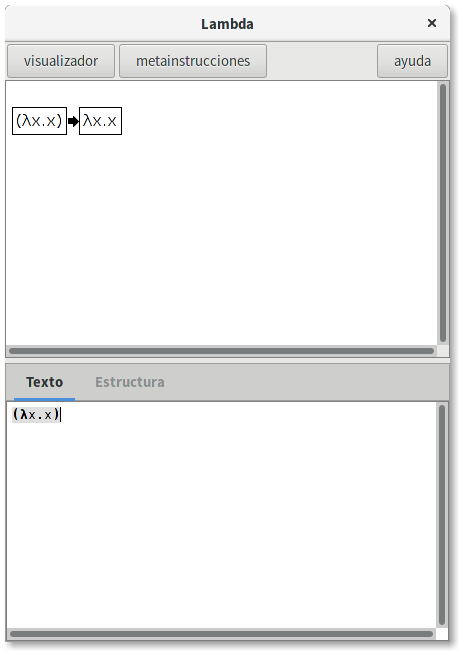
\includegraphics[scale=.22]{pimg/ventana-principal.png}\hspace{1cm}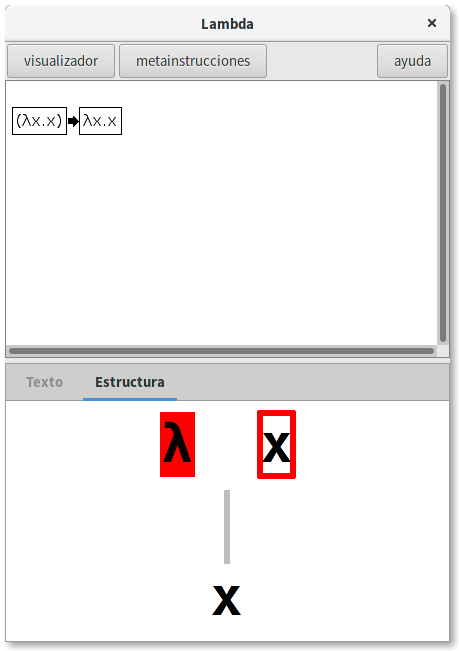
\includegraphics[scale=.22]{pimg/ventana-principal-2.png}
    }\only<2>{
      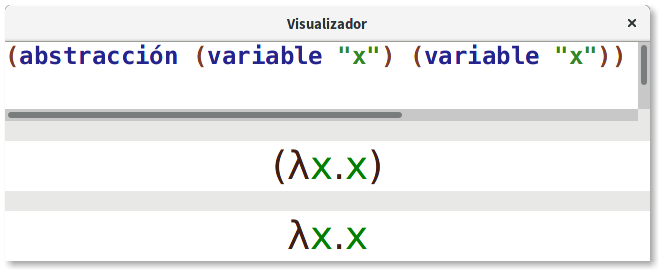
\includegraphics[scale=.22]{pimg/visualizador.png}

      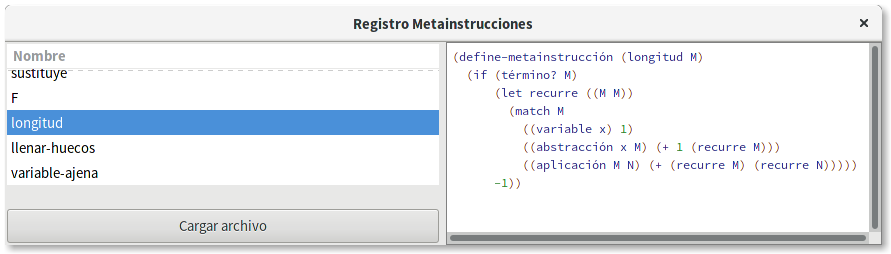
\includegraphics[scale=.22]{pimg/registro.png}
    }
  \end{center}
  
\end{frame}

\begin{frame}[standout]
  \vfill
  {\Huge ¿Preguntas?}
  \vfill
  {
    \small
    El código fuente de esta presentación, la tesis y los programas se pueden descargar de

    \url{github.com/eduardoacye/tesis}

    \vfill
    
    \ccbysa

    {\footnotesize (Atribución-Licenciamiento Recíproco)}
  }
\end{frame}

% \appendix

% \begin{frame}[allowframebreaks]
%   \frametitle{Referencias}
  
% \end{frame}

\end{document}


%%% Local Variables:
%%% mode: LaTeX
%%% TeX-master: t
%%% End:
